\documentclass[aps,prl,reprint,superscriptaddress,nofootinbib]{revtex4-2}
\usepackage[T1]{fontenc}
\usepackage[utf8]{inputenc}
\usepackage{amsmath,amssymb,amsfonts,bm}
\usepackage{graphicx}
\usepackage{booktabs}
\usepackage{hyperref}
\usepackage{tikz}
\newcommand{\dd}{\mathrm{d}}
\newcommand{\MSbar}{\overline{\mathrm{MS}}}
\newcommand{\GeV}{\,\mathrm{GeV}}
\newcommand{\Jcas}{J}
\newcommand{\xp}{x_+}
\newcommand{\xm}{x_-}
\newcommand{\sPole}{s^2_{\rm pole}}
\newcommand{\sdV}{s^2_{\rm dV}}
\newcommand{\GSM}{G_{\rm SM}}


\begin{document}

\title{Electroweak couplings fixed by Kaluza--Klein moduli:\\
a parameter-free weak mixing angle and fine-structure constant}

\author{Alejandro Rivero}
\affiliation{EUPT, Universidad de Zaragoza}

\date{\today}

\begin{abstract}
The weak mixing angle and the fine-structure constant are independent inputs of
the Standard Model. We argue they are fixed by the geometry of electroweak
symmetry breaking. Kaluza--Klein reduction makes a gauge coupling a function of
the compactification size but leaves that size a free modulus, so the coupling
is geometric yet undetermined. We propose that the order parameter of
electroweak breaking is the field that stabilizes the modulus: one act of
breaking gives the gauge bosons their mass and fixes the size, and with it the
couplings. Fermion chirality forces the construction to the ten-dimensional
point of an interpolation between an unbroken eleven-dimensional endpoint and a
broken nine-dimensional one, evading the chirality obstruction of
eleven-dimensional supergravity. A breaking operator at each internal level
realizes this: its upper branch is the gauge sector, fixing $\sin^2\theta$ as a
ratio; its lower branch is the order parameter, which---given the assignments stated
below---fixes $\alpha$ as a pure number, $1/\alpha=135.3$, in the infrared. The parameter-free numerical
agreement is the evidence.
\end{abstract}

\maketitle

\textit{The claim.}---The electroweak sector carries two dimensionless
parameters, the weak mixing angle $\sin^2\theta$ and the fine-structure constant
$\alpha$, taken as measured inputs. We argue that the geometry of symmetry
breaking fixes both, through a single mechanism: the field that breaks the
electroweak symmetry is the field that fixes the size of the compact dimensions. The argument runs in five steps, and the
numbers enter only at the end, as its test.

\textit{Kaluza--Klein makes a coupling geometric, then leaves it free.}---In a
Kaluza--Klein theory the four-dimensional gauge couplings are determined by the
internal geometry. Witten's analysis states it plainly: the couplings scale as a
power of $1/(M_pR)$, with $R$ the radius of the extra dimensions, so the coupling
\emph{is} the size \cite{WittenKK1981}. The same analysis states the obstruction:
``the field equations do not determine the radius of the circle,'' which appears
as ``a massless scalar degree of freedom'' \cite{WittenKK1981}. The size is a
modulus. A Kaluza--Klein theory therefore predicts a coupling only once something
fixes that modulus. Identifying what fixes it is the content of this Letter.

\textit{Chirality points to ten dimensions.}---The unbroken gauge group
$SU(3)\times SU(2)\times U(1)$ requires seven internal dimensions, hence total
$D=11$; but Witten proved that this seven-dimensional compactification cannot
produce chiral fermions with the correct quantum numbers \cite{WittenKK1981}. The
physical world is therefore not at that endpoint. Electroweak breaking moves the
system along the interpolation that ends, when the breaking is complete, at
$SU(3)\times U(1)_{\rm em}$ in five internal dimensions ($D=9$). Its interior
point sits at six internal dimensions, $D=10$---the critical dimension of the
superstring, where chiral fermions are standard. Witten's no-go constrains the
$D=11$ endpoint and leaves a $D=10$ interior unconstrained. We take this as
motivation only: the interpolation is heuristic, with no interpolating field
exhibited through a noninteger dimension, yet it places the construction at $D=10$, where
the string (Regge) excitations and the relevant moduli also live.

\textit{Breaking is moduli stabilization.}---At each internal level, labelled by
the Laplacian eigenvalue $J=s(s+1)$, a gauge mode and an order-parameter mode
mix into one operator,
\begin{equation}
Q(J)=\mu^2\begin{pmatrix}0&\sqrt J\\ \sqrt J&-J\end{pmatrix},
\qquad
x_\pm(J)=\tfrac12\!\left(-J\pm\sqrt{J^2+4J}\right),
\label{eq:operator}
\end{equation}
with eigenvalues $\mu^2x_\pm$ and the invariant $x_+x_-=-J$, equivalently
$M_+^2M_-^2=-\mu^4J$: one operator sets both branches together. The family
$x^2+Ax-A=0$ has golden roots at $A=1$, and \eqref{eq:operator} is its
angular-momentum member $A=s(s+1)$, so the golden ratio is the special level
$s=1/\varphi$. The off-diagonal
$\sqrt J$ is
geometric: the exact one-form $d\phi$ built from a level-$J$ scalar satisfies
$\|d\phi\|^2=J\|\phi\|^2$, so the gauge--scalar mixing is $\sqrt J$. This off-diagonal is the supercharge of
an $N=2$ supersymmetric quantum mechanics: with the exterior derivative $d$ and
its adjoint $\delta$ as supercharges, $\{d,\delta\}=\Delta$ is the Hodge
Laplacian, pairing the scalar and vector modes degenerately at eigenvalue $J$
\cite{WittenMorse1982}; the diagonal $-J$ breaks this supersymmetry and lifts the
degeneracy, so the two branches are the split would-be superpartners---a broken
$N=2$ supersymmetric quantum mechanics, the operator content of the original
``susy-like'' degeneration \cite{Rivero2006}. The upper
branch $x_+>0$ is the massive gauge mode; the lower branch $x_-<0$ is tachyonic.
A negative mass squared is not a pathology on a compact internal space: such a
mode is admissible when it respects the Breitenlohner--Freedman bound, and a
stabilized negative mode is what selects a new vacuum radius, as in the
squashed-sphere deformations of Kaluza--Klein supergravity
\cite{DuffNilssonPope1986,BreitenlohnerFreedman1982}. Its condensation \emph{is}
the symmetry breaking and the stabilization of the modulus: the lower branch is
the order parameter that fixes $R$. That the electroweak sector and the
compactification modulus are tied in this way is established in extra-dimensional
models, where the Higgs and the radion mix or the Higgs itself stabilizes the
radius \cite{Bucci2004,HabaOda2011}, and in gauge-Higgs unification, where the
order parameter is a component of the higher-dimensional gauge field with its
potential fixed by the compactification \cite{SalamStrathdee1982,Hosotani1983}.
We adopt, as a hypothesis, the strongest form of this link, in which the order
parameter \emph{is} the stabilizer. One operator then does both jobs---it gives
the gauge bosons mass and fixes the size that Witten left free.

\textit{Hence the couplings.}---Assign the upper branch to the massive vectors,
$M_V^2=\mu^2x_+(J_V)$, with the charged sector at the doublet value $J=\tfrac34$ and the neutral sector
at the adjoint value $J=2$ (the label $s$ in $J=s(s+1)$ is an internal
representation index, distinct from the Lorentz spin and the Regge level). The mixing
angle is then a ratio within this one branch,
\begin{equation}
\sin^2\theta=1-\frac{M_W^2}{M_Z^2}=1-\frac{x_+(3/4)}{x_+(2)}=0.223101 .
\label{eq:sin2}
\end{equation}
Once the lower branch fixes $R$, the gauge coupling is no longer free. Because
the gauge mass $M_W$ and the order parameter $v=\sqrt2\,M_-(2)$ are eigenvalues
of the \emph{same} operator, both proportional to $\mu$, the scale cancels:
\begin{align}
g^2&=\frac{4M_W^2}{v^2}=x_+(3/4)\,x_+(2),\nonumber\\
\frac1\alpha&=\frac{4\pi}{x_+(3/4)\,[x_+(2)-x_+(3/4)]}=135.3 .
\label{eq:alpha}
\end{align}
The coupling is read where the modulus is fixed---the compact, infrared
scale---so it should match the running coupling there, well below $M_Z$. The measured
$1/\alpha$ runs from $137.036$ at zero momentum to $127.955$ at $M_Z$
\cite{PDG2025}; the value $135.3$ sits at the low-energy end, in the
few-GeV/hadronic region, where the comparison carries the hadronic
vacuum-polarization uncertainty \cite{Jegerlehner2019}. The picture places
$\alpha$ in the infrared, far from $M_Z$; the precise scale awaits that
uncertainty.

\textit{One scale, two dual branches.}---The defining feature of $Q(J)$ is that
its dimensionless eigenvalues have equal trace and determinant,
$x_++x_-=x_+x_-=-J$. Their reciprocals therefore partition unity,
$1/x_++1/x_-=1$, that is
\begin{equation}
\frac{1}{M_+^2}+\frac{1}{M_-^2}=\frac1{\mu^2},
\qquad
\operatorname{tr}Q(J)^{-1}=\frac1{\mu^2},
\label{eq:reciprocal}
\end{equation}
for every level: the inverse operator carries a level-independent trace set by
the one scale. Each gauge mass combines in parallel with its order-parameter
partner to $\mu^2$; the $Z$ slot gives $M_Z^2$ as the parallel combination of
$\mu^2$ and $M_-^2(2)$. The two branches are exchanged by the inversion
$x\to-J/x$, equivalently $M^2\to-\mu^4J/M^2$, an ultraviolet--infrared duality
that maps the light gauge branch onto the heavy order-parameter branch and is
fixed by the same trace--determinant condition. The construction is in this sense
self-dual at each level, the gauge and order-parameter sectors being two faces of
one operator. The large-level behaviour identifies those faces against the spin
$s$: $M_+\to\mu$ is bounded (a point, the $p{=}0$ rotating-brane law
$M\sim\text{const}$), while $M_-\propto s$ (since $|x_-|\to J=s(s+1)$), the
$p\to\infty$ space-filling case. The inversion exchanges a point-like (D0) and a
space-filling branch, an all-Dirichlet/all-Neumann T-dual pair.

\begin{table}[t]
\caption{What the construction derives versus what it assigns. The derived rows
are exact algebra; the assigned rows are the Kaluza--Klein identifications a
reduced-action derivation must supply.}
\label{tab:ledger}
\begin{ruledtabular}
\footnotesize
\begin{tabular}{ll}
Derived (algebra) & Assigned (KK identification) \\
\colrule
$x^2+Jx-J=0$, roots $x_\pm$ & operator $Q(J)$ from a $D{=}10$ reduction \\
$x_+x_-=x_++x_-=-J$ & sign of the $-J$ entry (negative mode) \\
$1/M_+^2+1/M_-^2=1/\mu^2$ & upper branch $\leftrightarrow$ gauge bosons \\
inversion $x\to-J/x$ & $(J_W,J_Z)=(3/4,2)$ \\
$g^2=x_+(3/4)\,x_+(2)$, $\sin^2\theta$, $\alpha$ & $v=\sqrt2\,M_-(2)$ \\
\end{tabular}
\end{ruledtabular}
\end{table}

\textit{Evidence.}---The claim is the mechanism; the numbers test it. First,
\eqref{eq:sin2} equals the on-shell value $1-M_W^2/M_Z^2=0.22320$ from
$M_W=80.369$, $M_Z=91.188\GeV$ \cite{PDG2025} to $0.04\%$; it is the pole-mass
angle, distinct from the effective ($0.23155$) and $\MSbar$ ($0.23129$)
definitions \cite{MartinRobertson2025}. Second, fixing the one scale by
$M_Z^2=\mu^2x_+(2)$ gives $\mu=106.578\GeV$ and the spectrum of
Table~\ref{tab:spectrum}: the upper branch returns $W$, the lower branch returns
scalar and fermion scales near the Higgs and top and the vacuum, each within a
percent---from one input. Third, the upper branch continues to higher levels:
$s=3/2$ places a state at $M_+=\mu\sqrt{x_+(15/4)}=96.5\GeV$. The upper branch
carries bosons, so this is a further neutral boson; were it the reported
$\sim95\GeV$ diphoton feature \cite{Biekotter2023} it would be neutral and
spin-$0$, which fixes its quantum numbers. We assign it no electric charge: a
single chiral charged state would not complete a Dirac fermion under the
vector-like electromagnetic $U(1)$, and a $\gamma\gamma$ resonance is in any case
neutral.

\begin{table}[t]
\caption{Both branches from one input, $\mu=106.578\GeV$ fixed by $M_Z$.
Reference values from \cite{PDG2025}.}
\label{tab:spectrum}
\begin{ruledtabular}
\begin{tabular}{lccc}
 & level & branch [GeV] & reference [GeV] \\
\colrule
$W$ (gauge)        & $x_+(3/4)$ & $80.375$  & $80.369$ \\
$Z$ (gauge)        & $x_+(2)$   & $91.188$  & $91.188$ (input) \\
order param.\ (h?) & $x_-(3/4)$ & $122.39$  & $125.20$ \\
order param.\ (t?) & $x_-(2)$   & $176.16$  & $172.57$ \\
vacuum $v$         & --         & $249.13$  & $246.22$ \\
\end{tabular}
\end{ruledtabular}
\end{table}

\begin{figure}[t]
\centering
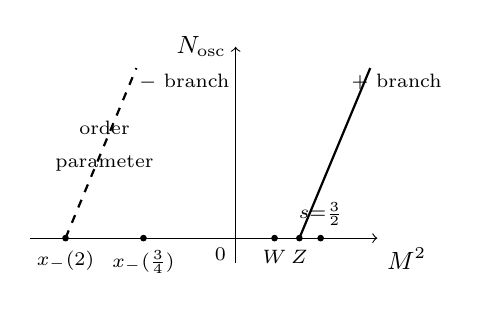
\begin{tikzpicture}[scale=0.9]
  \draw[->] (-2.9,0) -- (2.0,0) node[below right] {\small $M^2$};
  \draw[->] (0,-0.35) -- (0,2.7) node[left] {\small $N_{\rm osc}$};
  \node[below left] at (0,0) {\scriptsize $0$};
  \draw[thick] (0.9,0) -- (1.9,2.4);
  \node[right] at (1.5,2.2) {\scriptsize $+$ branch};
  \draw[thick,dashed] (-2.4,0) -- (-1.4,2.4);
  \node[right] at (-1.5,2.2) {\scriptsize $-$ branch};
  \filldraw (0.55,0) circle (1.1pt) node[below=1pt] {\scriptsize $W$};
  \filldraw (0.9,0) circle (1.1pt) node[below=1pt] {\scriptsize $Z$};
  \filldraw (1.2,0) circle (1.1pt) node[above=1pt] {\scriptsize $s{=}\tfrac32$};
  \filldraw (-1.3,0) circle (1.1pt) node[below=1pt] {\scriptsize $x_-(\tfrac34)$};
  \filldraw (-2.4,0) circle (1.1pt) node[below=1pt] {\scriptsize $x_-(2)$};
  \node[align=center] at (-1.85,1.3) {\scriptsize order\\\scriptsize parameter};
\end{tikzpicture}
\caption{Schematic Chew--Frautschi reading: the two branches are the
$N_{\rm osc}=0$ intercepts of common-slope trajectories
$M^2_{N_{\rm osc},j,\pm}=\mu^2x_\pm(j(j+1))+N_{\rm osc}/\alpha'$. Positive
intercepts carry the gauge bosons ($W$, $Z$) and higher neutral states; negative
(tachyonic) intercepts carry the order-parameter scales. Not to scale.}
\label{fig:regge}
\end{figure}

\textit{Discussion.}---The result is the mechanism: electroweak symmetry breaking
is Kaluza--Klein moduli stabilization, so the order parameter that breaks the
symmetry fixes the compactification and, with it, the two dimensionless
couplings; chirality places the construction in ten dimensions; and $\alpha$ is
an infrared quantity because it is read where the modulus is fixed. The numbers
are the evidence that the mechanism is real.

Two derivations remain, and we state them as such. The internal six-manifold
whose mode reduction yields \eqref{eq:operator} is not identified here: the
geometric mixing $\sqrt J$ and the massless gauge entry follow from the Hodge
structure, while the tachyonic entry $-J$ requires the internal curvature to
supply the order-parameter mass at each level. Equal trace and determinant force
$(\text{off-diagonal})^2=-(\text{lower entry})$, so $\sqrt J$ and $-J$ are one
internal datum, the Laplacian eigenvalue and its root; the open input is the
single sign that makes the order-parameter mode tachyonic, a
Breitenlohner--Freedman-admissible negative mode on a squashed internal space
such as $S^3=SU(2)$, whose Casimir is $j(j+1)$. The half-integer slot
$J=3/4$ ($s=\tfrac12$) requires the spinor harmonics of $S^3=SU(2)$, absent on
the coset $S^2$, which carries only integer $l$. And the assignment
$(J_W,J_Z)=(\tfrac34,2)$ remains to be derived from the gauge-Higgs reduction.
Each level extends to a common-slope Regge trajectory
$M^2_{N_{\rm osc},j,\pm}=\mu^2x_\pm(j(j+1))+N_{\rm osc}/\alpha'$, with the sector
label $j$, the oscillator level $N_{\rm osc}$, and the physical spin kept
distinct and the present states at $N_{\rm osc}=0$ (Fig.~\ref{fig:regge})---the
string excitations of the same ten-dimensional compactification. This structure is developed in a
companion long version. The claim of this Letter stands on its own: the geometry that fixes the
extra dimensions fixes the electroweak couplings.

\begin{acknowledgments}
The construction originates in the de Vries--Rivero observation \cite{Rivero2006}.
\end{acknowledgments}

\bibliography{references}

\end{document}
